\documentclass[twoside]{homework}
\usepackage{graphicx}
\usepackage{mathtools}
\usepackage{float}
\usepackage{hyperref}
\DeclarePairedDelimiter\ceil{\lceil}{\rceil}
\DeclarePairedDelimiter\floor{\lfloor}{\rfloor}
\newcommand\Myperm[2][^n]{\prescript{#1\mkern-2.5mu}{}P_{#2}}

\studname{Name: Geraldi Dzakwan (gd2551). Discussants: Deka (da2897), Patricia (pk2618)}
% \studmail{Discussants: Deka (da2897), Patricia (pk2618)}
\coursename{COMS W4771: Machine Learning (sec:001)}
\hwNo{3}

\begin{document}
\maketitle

\section*{Problem 1}
\begin{itemize}
    \item [a.] Function name: \boldsymbol{compute\_min\_euclidean\_norm\_solution} in file p1/a1.py. This function will take feature matrix A, shape: (32, 256), and b, shape: (32), as the input. Thus, the feature map needs to be applied to the original A, shape: (32,1), before the function takes A as its input. Then, it computes the minimum Euclidean norm solution using the Moore Penrose inverse. This is as suggested in Problem 4. This function is called in a bigger function \boldsymbol{compute\_euclid} that also does other things like plotting the solution on test data. List of subfunctions/subroutines and external software libraries used:
    \begin{itemize}
        \item [1.] To transform the feature vector A of shape (32,1) to shape (32,256), subfunction \boldsymbol{transform\_feature} is used. This subfunction basically takes A and transform each row in A from dimension 1 to dimension 256 using the feature map described in the problem.
        \item [2.] Next, compute the Moore Penrose inverse of matrix A using the library \textbf{numpy.linalg.pinv}, numpy version: 1.15.1.
        \item [3.] Finally, return the minimum Euclidean solution as the multiplication (using numpy.dot) between the Moore Penrose inverse of A and the label vector b.
    \end{itemize}
    Additional note:
    \begin{itemize}
        \item [1.] Since A has full row rank, I also try to use another way to find the minimum Euclidean norm by using \boldsymbol{numpy.lstsq} and it yields the same result. The differences of the Euclidean norm of the solution and the error rate on training data for both methods are less than 1e-10.
        \item [2.] To use numpy lstsq, two inputs are needed, which are $A^TA$ of shape (256, 256) and $A^Tb$ of shape (256). They are respectively the left hand side (excluding the solution $w$) and the right hand side of the normal equation.
        \item [3.] But, the default method used in the function \textit{compute\_min\_euclidean\_norm\_solution} is the Moore Penrose inverse as it can accommodate all types of matrices, including those that don't have full row rank. This is implemented in the function as default param: \textit{use\_pinv=True}.
    \end{itemize}
    \item [b.] The plot for $(\~x_i,\hat{f}_{Euclid}(\~x_i))$ for $i=1,...,m$ is as below (Figure 1). The points are depicted as dots with black edge and white fill. The pink lines connect consecutive dots/points, e.g. $\~x_1 \text{ to } \~x_2, \~x_2 \text{ to } \~x_3$, etc. The plotted points are very scattered.
        \begin{figure}[H]
            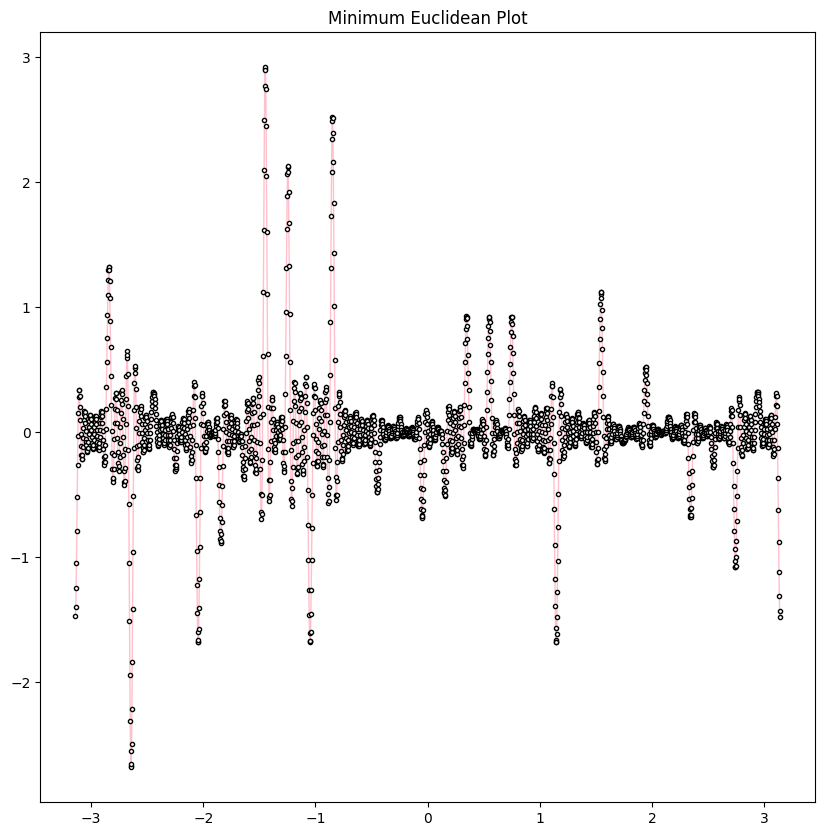
\includegraphics[scale=0.6]{1a.png}
            \caption{Minimum Euclidean Plot}
            \label{fig:minimum_euclidean_plot}
        \end{figure}
    \newpage
    \item [c.] To get the weighted minimum Euclidean norm, I use the same function as the function used in Part (a): \boldsymbol{compute\_min\_euclidean\_norm\_solution}. The difference is that I make some changes to the input feature matrix A, shape: (32, 256), and b, shape: (32). The changes are as below:
    \begin{itemize}
        \item [1.] I create a diagonal matrix of shape (256, 256) in which the diagonal element represent the square root of the weights, i.e. the diagonal element at row $j$, $j$ starts from zero, will have the value of $\ceil{(j+1)/2}$. Denote this by V.
        \item [2.] Matrix A will be stacked with the diagonal matrix with the diagonal matrix is being placed at the bottom. The new matrix A, say $\~A$, will have the shape of (32+256, 256). This is done using \boldsymbol{np.vstack}.
        \item [3.] The label vector b is padded with zero vectors of size 256 so that the shape becomes (32+256). Call this \~b.
    \end{itemize}
    When those changes are applied, we will obtain a new covariance matrix, say $\~A^T\~A$, where:
    $$\~A^T\~A=(A^TA + V^2)$$
    $V^2$ is a diagonal matrix in which the diagonal element represent the weights, i.e. the diagonal element at row $j$, $j$ starts from zero, will have the value of $\ceil{(j+1)/2}^2$. This is inspired by ridge regression where the regularization is done by padding A with $\sqrt{\lambda}I$. The difference in this case is we use weighted diagonal matrix to replace the diagonal matrix $\sqrt{\lambda}I$.
    \newline\newline
    To check the correctness of my procedure, I print the first and last 16 elements of the solution and check their values. It is as below:
    \begin{itemize}
        \item [1.] First 16 elements: [ 0.4032034  -0.06122629 -0.23717626 -0.19003089 -0.19338498  0.12254494  0.05226381  0.27718176 -0.05410099  0.00179812 -0.10968115     -0.07202143  -0.07760895  0.0042153   0.0720863   0.04318911]
        \item [2.] Last 16 elements: [-8.04757022e-05  1.50789327e-06  2.09760474e-05 -3.10685887e-04 -1.22647149e-04 -4.49403833e-05 -5.42573418e-05  4.60438734e-05 2.82446691e-05  8.82269746e-06  1.32173310e-05 -8.67592810e-06 2.37082353e-05  1.22843870e-06 -6.58580580e-05 -4.84817254e-05]
    \end{itemize}
    It can be seen that the last 16 elements are way smaller than the first 16 elements. This makes sense since we try to minimize the weighted Euclidean norm and the last 16 elements have way bigger weights: $\ceil{240/2}, ..., \ceil{256/2}$, than the first 16 elements: $\ceil{1/2}, ..., \ceil{16/2}$.
    \newpage
    \item [d.] The plot for $(\~x_i,\hat{f}_{weighted}(\~x_i))$ for $i=1,...,m$ is as below (Figure 2). The plotted points form dense lines, they don't scatter like the plot for minimum Euclidean norm. The pink lines are not visible because consecutive points are very close to each other.
        \begin{figure}[H]
            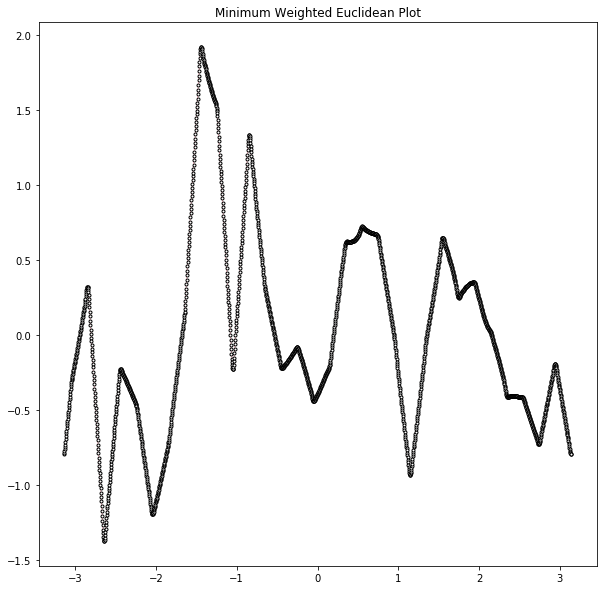
\includegraphics[scale=0.6]{1b.png}
            \caption{Minimum Weighted Euclidean Plot}
            \label{fig:minimum_weighted_euclidean_plot}
        \end{figure}
    \newpage
    \item [e.] The plot for $(\~x_i,\hat{f}_{Dantzig}(\~x_i))$ for $i=1,...,m$ is as below (Figure 3). This looks like the plot for the minimum weighted Euclidean norm, except that this plot somewhat represents higher polynomial order with its curves. The lines are also not as dense as the minimum weighted Euclidean norm, especially for $\~x<0$, i.e. the left half of the plot. Thus, we can still see the pink lines there.
        \begin{figure}[H]
            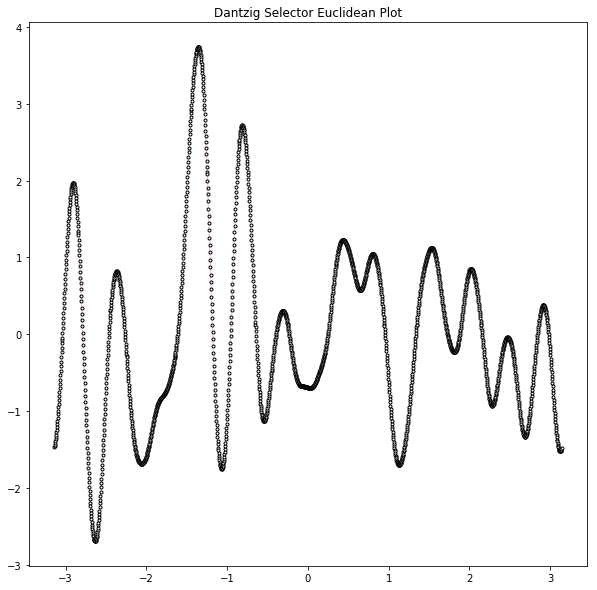
\includegraphics[scale=0.6]{1c.png}
            \caption{Dantzig Selector Euclidean Plot}
            \label{fig:dantzig_selector_euclidean_plot}
        \end{figure}
    \newpage
    \item [f.] When counting non-zero entries, I consider entries which absolute value is less than $1e-15$ to be zero entries.
    \begin{itemize}
        \item [1.] Number of non-zero entries in $\hat{w}_{Euclid}$: 0
        \item [2.] Number of non-zero entries in $\hat{w}_{weighted}$: 0
        \item [3.] Number of non-zero entries in $\hat{w}_{Dantzig}$: 222
    \end{itemize}
    For Dantzig selector, the number of non-zero entries may differ for different parameters used when calling \textbf{scipy.optimize.linprog}. In my experiment, I use \textbf{scipy version 1.3.1} and \textbf{"revised simplex"} as the optimization method. But, the number of nonzero entries are generally above 200.
    \item [g.]
\end{itemize}
\newpage

\section*{Problem 2}
\begin{itemize}
    \item [a.] The performance of the 20-class Naive Bayes classifier $\hat{f}$ on the full 20 Newsgroup data set is as below.
        \begin{itemize}
            \item [1.] Training error rate: \boldsymbol{0.21581329310497827}
            \item [2.] Test error rate: \boldsymbol{0.3769487008660893}
        \end{itemize}
    \item [b.] The performance of the binary Naive Bayes classifier on the modified 20 Newsgroup data set is as below.
        \begin{itemize}
            \item [1.] Training error rate: \boldsymbol{0.05779392338177015}
            \item [2.] Test error rate: \boldsymbol{0.13138324243926625}
        \end{itemize}
    \item [c.] The ordered lists are listed in Table 1 and Table 2 below. Both are sorted descendingly based on their weight absolute value.  $vocab\_index$ is in range $[0, 61188)$.
        \begin{itemize}
            \item [1.] Most positive words (top 20) and their weights descendingly sorted.
            \begin{table}[h!]
                \centering
                \begin{tabular}{||c c c c||}
                    \hline
                    $no$ & $vocab\_index$ & $word$ & $weight$ \\ [1ex]
                    \hline\hline
                    1 & 38732 & firearms & 4.684503228539178\\
                    \hline
                    2 & 20611 & occupied & 4.5486749575136685\\
                    \hline
                    3 & 48903 & israelis & 4.407062712835207\\
                    \hline
                    4 & 49311 & serdar & 4.394416055789522\\
                    \hline
                    5 & 49312 & argic & 4.394416055789522\\
                    \hline
                    6 & 49313 & ohanus & 4.230244601288161\\
                    \hline
                    7 & 49314 & appressian & 4.230244601288161\\
                    \hline
                    8 & 49316 & sahak & 4.230244601288161\\
                    \hline
                    9 & 49317 & melkonian & 4.230244601288161\\
                    \hline
                    10 & 45378 & villages & 4.215395293623014\\
                    \hline
                    11 & 49216 & cramer & 4.054622073035262\\
                    \hline
                    12 & 49315 & armenia & 4.038936035689443\\
                    \hline
                    13 & 50290 & cpr & 4.037155106460034\\
                    \hline
                    14 & 49252 & sdpa & 4.019401259954519\\
                    \hline
                    15 & 39353 & optilink & 4.001350538635606\\
                    \hline
                    16 & 28710 & handgun & 4.001350538635606\\
                    \hline
                    17 & 45016 & palestine & 4.001350538635606\\
                    \hline
                    18 & 47918 & firearm & 3.9829924168960074\\
                    \hline
                    19 & 12178 & budget & 3.906254594442897\\
                    \hline
                    20 & 47471 & arabs & 3.854840727802684\\
                    \hline
                \end{tabular}
                \caption{Top 20 Positive Words}
                \label{table:1}
            \end{table}
            \newpage
            \item [2.] Most negative words (top 20) and their weights descendingly sorted.
            \begin{table}[h!]
                \centering
                \begin{tabular}{||c c c c||}
                    \hline
                    $no$ & $vocab\_index$ & $word$ & $weight$ \\ [1ex]
                    \hline\hline
                    1 & 45948 & athos & -5.181568936831565\\
                    \hline
                    2 & 2 & atheism & -4.795686699947933\\
                    \hline
                    3 & 877 & atheists & -4.7642014773182675\\
                    \hline
                    4 & 46033 & clh & -4.7318384934967765\\
                    \hline
                    5 & 2234 & teachings & -4.419101733948125\\
                    \hline
                    6 & 2604 & revelation & -4.213637631942487\\
                    \hline
                    7 & 3548 & testament & -4.178305464858287\\
                    \hline
                    8 & 896 & livesey & -4.160199181208549\\
                    \hline
                    9 & 9 & atheist & -4.152563313255224\\
                    \hline
                    10 & 897 & solntze & -4.123053546615284\\
                    \hline
                    11 & 898 & wpd & -4.123053546615284\\
                    \hline
                    12 & 7886 & scriptures & -4.084586757943714\\
                    \hline
                    13 & 1973 & theology & -4.06482656579093\\
                    \hline
                    14 & 2883 & believers & -4.044696989331064\\
                    \hline
                    15 & 7017 & alink & -3.9819409279865594\\
                    \hline
                    16 & 7018 & ksand & -3.9819409279865594\\
                    \hline
                    17 & 1880 & benedikt & -3.93796287361363\\
                    \hline
                    18 & 1923 & jesus & -3.934746865891957\\
                    \hline
                    19 & 3919 & prophet & -3.8920946802110823\\
                    \hline
                    20 & 3301 & mozumder & -3.8920946802110823\\
                    \hline
                \end{tabular}
                \caption{Top 20 Negative Words}
                \label{table:2}
            \end{table}
        \end{itemize}
\end{itemize}
\clearpage

\section*{Problem 3}
\begin{itemize}
    \item [a.] The number of iterations $T$ needed to reach zero training rate is \boldsymbol{1194}. In this case, the iteration starts from zero, i.e. when $t=0$, $w=w^{(0)}=0$.
    \item [b.] Test error rate of $w^{(T)}$, i.e $w^{(1194)}$ is \boldsymbol{0.08329201784828955}.
    \item [c.] The ordered lists are listed in Table 3 and Table 4 below. Both are sorted descendingly based on their weight absolute value.  $vocab\_index$ is in range $[0, 61188)$.
        \begin{itemize}
            \item [1.] Most positive words (top 20) and their weights descendingly sorted.
            \begin{table}[h!]
                \centering
                \begin{tabular}{||c c c c||}
                    \hline
                    $no$ & $vocab\_index$ & $word$ & $weight$ \\ [1ex]
                    \hline\hline
                    1 & 4751 & israel & 1.1811551891717107\\
                    \hline
                    2 & 1144 & gun & 1.0983107882823702\\
                    \hline
                    3 & 5687 & clinton & 0.930665329319725\\
                    \hline
                    4 & 2183 & politics & 0.9289544423611378\\
                    \hline
                    5 & 87 & american & 0.9057536874334365\\
                    \hline
                    6 & 2227 & government & 0.8737978481876671\\
                    \hline
                    7 & 3831 & news & 0.8362673178451754\\
                    \hline
                    8 & 2190 & guns & 0.8233855149924485\\
                    \hline
                    9 & 32214 & kaldis & 0.788478406105581\\
                    \hline
                    10 & 1738 & rights & 0.7847489417090874\\
                    \hline
                    11 & 5116 & israeli & 0.7713478327943094\\
                    \hline
                    12 & 9054 & theodore & 0.7353256505192912\\
                    \hline
                    13 & 1505 & mr & 0.6656585405248127\\
                    \hline
                    14 & 1160 & getting & 0.6512600848339959\\
                    \hline
                    15 & 266 & white & 0.6419091028730181\\
                    \hline
                    16 & 9930 & weapons & 0.6362051644909561\\
                    \hline
                    17 & 3384 & president & 0.6301780205108527\\
                    \hline
                    18 & 1501 & country & 0.6263872024735501\\
                    \hline
                    19 & 2294 & jews & 0.6234934161118683\\
                    \hline
                    20 & 38732 & firearms & 0.6227264471566076\\
                    \hline
                \end{tabular}
                \caption{Top 20 Positive Words}
                \label{table:3}
            \end{table}
            \newpage
            \item [2.] Most negative words (top 20) and their weights descendingly sorted.
            \begin{table}[h!]
                \centering
                \begin{tabular}{||c c c c||}
                    \hline
                    $no$ & $vocab\_index$ & $word$ & $weight$ \\ [1ex]
                    \hline\hline
                    1 & 315 & god & -1.8612543247469517\\
                \hline
                2 & 94 & bible & -1.4021643477777477\\
                \hline
                3 & 425 & christian & -1.3916783336359537\\
                \hline
                4 & 1923 & jesus & -1.3227597977024164\\
                \hline
                5 & 16 & religion & -1.1053169910011855\\
                \hline
                6 & 892 & keith & -1.0913660874572892\\
                \hline
                7 & 45 & christians & -1.0091501586855463\\
                \hline
                8 & 1931 & lord & -0.9952944263553888\\
                \hline
                9 & 275 & church & -0.9893978622339166\\
                \hline
                10 & 118 & james & -0.9518221157839706\\
                \hline
                11 & 45948 & athos & -0.8934685984660959\\
                \hline
                12 & 363 & christianity & -0.892301384230667\\
                \hline
                13 & 488 & christ & -0.8499905829531106\\
                \hline
                14 & 2 & atheism & -0.7755878085259651\\
                \hline
                15 & 1095 & kent & -0.7443617468611161\\
                \hline
                16 & 900 & jon & -0.7400024779543952\\
                \hline
                17 & 768 & mathew & -0.7323655192354515\\
                \hline
                18 & 3424 & koresh & -0.729462198687837\\
                \hline
                19 & 592 & religious & -0.7208049814283887\\
                \hline
                20 & 853 & jim & -0.7027838278194898\\
                \hline
                \end{tabular}
                \caption{Top 20 Negative Words}
                \label{table:4}
            \end{table}
        \end{itemize}
\end{itemize}
\clearpage

\section*{Problem 4}
\begin{itemize}
    \item [a.] We know that $\lambda$ is the non-zero eigenvalue of $A^TA$ with the corresponding eigenvector $v$. Then, the suitable equation would be:
    $$A^TAv = {\lambda}v$$
    Multiply both side by $A$:
    $$AA^TAv = A{\lambda}v$$
    $$AA^T(Av) = {\lambda}(Av) \text{ ... Eq. 1}$$
    The above equation shows that $\lambda$ is also the non-zero eigenvalue of $AA^T$ with the corresponding eigenvector $Av$.
    \item[b.] We need to proof that $v$ is in the null space of $A$. It means that we need to proof the following:
    $$Av=0$$
    Let's inspect the length ($l_2$ norm) of vector $Av$:
    $$ \lVert Av \rVert_2^2 = (Av)^TAv$$
    $$ \lVert Av \rVert_2^2 = v^TA^TAv$$
    $$ \lVert Av \rVert_2^2 = v^T(A^TAv)$$
    We know that $v$ is the eigenvector of $A^TA$, then we can replace it with ${\lambda}v$:
    $$ \lVert Av \rVert_2^2 = v^T({\lambda}v) \text{ ... Eq. 2}$$
    Since ${\lambda}=0$ in this case, then:
    $$ \lVert Av \rVert_2^2 = 0$$
    We know that only zero vector has $l_2$ norm of zero, then it is proved that:
    $$Av=0$$
    \item[c.] We know from Part (a) that any non-zero eigenvalues of $A^TA$ are also the eigenvalues of $AA^T$. So, to proof that $A^TA$ has the same eigenvalues as $AA^T$, then we also need to proof that any non-zero eigenvalues of $AA^T$ are also the eigenvalues of $A^TA$. Suppose $v$ is the eigenvector of $AA^T$ that corresponds with non-zero eigenvalue $\lambda$. We first start the following equation:
    $$AA^Tv={\lambda}v$$
    Multiply both side with $A^T$:
    $$A^TAA^Tv=A^T{\lambda}v$$
    $$A^TA(A^Tv)={\lambda}(A^Tv)$$
    The above equation shows that $\lambda$ is also the non-zero eigenvalue of $A^TA$ with the corresponding eigenvector $A^Tv$. Thus, from the above proof and proof in Part(a), it is proven that $A^TA$ has the same eigenvalues of $AA^T$.
    \item[d.] Let's rewrite $u_j$ as below:
    $$u_j = \frac{Av_j}{\lVert Av_j \rVert_2} = \frac{Av_j}{\sqrt{{v_j}^TA^TAv_j}} = \frac{Av_j}{\sqrt{{v_j}^T(A^TAv_j})} $$
    Since all $\lambda_j$ are strictly positive (non-zero), then we can use it as our denominator:
    $$u_j = \frac{Av_j}{\sqrt{{v_j}^T({\lambda}_jv_j)}} = \frac{Av_j}{\sqrt{{\lambda}_j({v_j}^Tv_j)}} = \frac{Av_j}{\sqrt{{\lambda}_j(\lVert v_j \rVert_2^2)}} $$
    Because $v_j$ is a normal vector, then:
    $$ u_j = \frac{Av_j}{\sqrt{{\lambda}_j(1)}} = \frac{Av_j}{\sqrt{{\lambda}_j}} \text{ ... Eq. 3}$$
    Suppose k follows $1\leq{j}<k\leq{r}$.
    Then, using Equation 3, for all pairs of $(j, k)$, we will have the dot product of $u_j^Tu_k$ as:
    $$ u_j^Tu_k = (\frac{(Av_j)^T}{\sqrt{{\lambda}_j}}) (\frac{Av_k}{\sqrt{{\lambda}_k}}) = \frac{v_j^T(A^TAv_k)}{\sqrt{{\lambda}_j\lambda_k}} $$
    $$ u_j^Tu_k =
    \frac{v_j^T{\lambda}_kv_k}{\sqrt{{\lambda}_j\lambda_k}} = \frac{{\lambda}_k(v_j^Tv_k)}{\sqrt{{\lambda}_j\lambda_k}} $$
    We know that $v_1, ..., v_d$ are orthonormal, then $v_1, ..., v_r$ are also orthonormal since it is a subset of $v_1, ..., v_d$. Hence, for all pairs of $(j,k)$, the dot product $v_j^Tv_k$ is zero and that makes:
    $$ u_j^Tu_k = \frac{{\lambda}_k(0)}{\sqrt{{\lambda}_j\lambda_k}} = 0$$
    Since for all pairs of $(j,k)$, we have $u_j^Tu_k = 0$, then it is proved that $u_1, ..., u_r$ are orthonormal.
    \item[e.]
    \item[f.] Using claim in Part (e), we need to show that:
    $$Aq_i=(\sum_{j=1}^r\sqrt{{\lambda}_j}u_j{v_j}^T)q_i \text{ for all } i=1,...,d$$
    If the above equation is proved, then A is proved to be the same as its decomposed value $\sum_{j=1}^r\sqrt{{\lambda}_j}u_j{v_j}^T$. $q_1, ..., q_d$ is a set of a linearly independent vector. In this case, we can use the set of orthonormal eigenvectors $v_1, ..., v_d$ as our $q_1, ..., q_d$ since it is also a set of linearly independent vector.
    \newline\newline
    We first start checking the left term $Aq_i\xrightarrow{}Av_i$. For each $i$, there will be two cases:
    \begin{itemize}
        \item[1.] For nonzero eigenvalues, i.e. for $1\leq{i}\leq{r}$. From Equation 3 in Part(d), we will have $ u_i = \frac{Av_i}{\sqrt{{\lambda}_i}} \xrightarrow{} Av_i = \sqrt{\lambda}_iu_i$.
        \item[2.] For zero eigenvalues, i.e. for $r<i\leq{d}$. We will have $ Av_i = 0$.
    \end{itemize}
    Next, we check the right term.
    $$(\sum_{j=1}^r\sqrt{{\lambda}_j}u_j{v_j}^T)q_i = (\sum_{j=1}^r\sqrt{{\lambda}_j}u_j{v_j}^T)v_i = \sum_{j=1}^r\sqrt{{\lambda}_j}(v_i^Tv_j)u_j$$
    For each $i$, again, there will be two cases:
    \begin{itemize}
        \item[1.] For nonzero eigenvalues, i.e. for $1\leq{i}\leq{r}$. Since $v_1, ..., v_r$ are orthonormal, then the dot product between $v_i$ and $v_j$ is zero except for $j=i$. Moreover, when $j=i$, $v_i^Tv_i=1^2=1$ since every $v$ is a unit vector. Thus, we will have: $$\sum_{j=1}^r\sqrt{{\lambda}_j}(v_i^Tv_j)u_j = (r-1)0 + \sqrt{\lambda_i}(v_i^Tv_i)u_i=\sqrt{\lambda_i}u_i$$
        \item[2.] For zero eigenvalues, i.e. for $r<i\leq{d}$. We will have $\sum_{j=1}^r\sqrt{{\lambda}_j}(v_i^Tv_j)u_j = 0$ as $v_i$ is a zero vector.
    \end{itemize}
    Finally, because $Av_i=(\sum_{j=1}^r\sqrt{{\lambda}_j}u_j{v_j}^T)v_i$ for $i=1,...,d$ where $v_1,...,v_d$ is a set of linearly independent vector, then it is proven that:
    $$A=\sum_{j=1}^r\sqrt{{\lambda}_j}u_j{v_j}^T$$.
\end{itemize}
\newpage

\section*{Problem 5}
\begin{itemize}
    \item [a.] The likelihood for $\theta$ given $Y$ would be:
    $$L(\theta|Y)=P(Y|\theta)=\frac{1}{(2\pi)^{n/2}|I|^{1/2}}\text{exp}(-\frac{1}{2}(Y-\theta)^TI^{-1}(Y-\theta))$$
    where $|I|^{1/2}=det(I)^{1/2}=1^{1/2}=1$ and $I^{-1}=I$. Thus:
    $$L(\theta|Y)=P(Y|\theta)=\frac{1}{(2\pi)^{n/2}}\text{exp}(-\frac{1}{2}(Y-\theta)^TI(Y-\theta))$$
    The log likelihood:
    $$\text{ln}L(\theta|Y)=\text{ln}(\frac{1}{(2\pi)^{n/2}}\text{exp}(-\frac{1}{2}(Y-\theta)^TI(Y-\theta)))$$
    $$\text{ln}L(\theta|Y)=\text{ln}({2\pi}^{-n/2})+\text{ln}(\text{exp}(-\frac{1}{2}(Y-\theta)^TI(Y-\theta)))$$
    $$\text{ln}L(\theta|Y)=-\frac{n}{2}\text{ln}(2\pi)-\frac{1}{2}(Y-\theta)^TI(Y-\theta)$$
    To find $\theta_{MLE}$, we take the first derivative w.r.t to $\theta$ and find $\theta$ that makes it zero:
    $$\frac{d}{d\theta}\text{ln}L(\theta|Y)=0$$
    $$\frac{d}{d\theta}(-\frac{n}{2}\text{ln}(2\pi)-\frac{1}{2}(Y-\theta)^TI(Y-\theta))=0$$
    $$0-(\frac{1}{2})\frac{d}{d\theta}((Y-\theta)^TI(Y-\theta))=0$$
    $$\frac{d}{d\theta}((Y-\theta)^TI(Y-\theta))=0$$
    We can use the fact that $\mathbf{ \frac{\partial w^T A w}{\partial w} = 2Aw}$ in this case since $w=(Y-\theta)$ is not dependent on $A=I$ and $I$ is an identity matrix that is symmetric. Then:
    $$2I(Y-\theta)=0 \xrightarrow{} 2(Y-\theta)=0 \xrightarrow{} Y-\theta=0$$
    Hence, the $\theta_{MLE}$ is
    $$\boldsymbol{\theta_{MLE}=Y=(y_1, y_2, ..., y_n)}$$
    \item [b.] The prior distribution ($\mu_i=0$, $\sigma^2_i=\tau$):
    $$P(\theta_i)=\frac{1}{\sigma_i\sqrt{2\pi}}\text{exp}(-\frac{(\theta_i-\mu_i)^2}{2\sigma_i^2})$$
    $$P(\theta_i)=\frac{1}{\sqrt{2\pi\tau}}\text{exp}(-\frac{\theta_i^2}{2\tau})$$
    The likelihood ($\mu_i=\theta_i$, $\sigma_i^2=1$):
    $$P(y_i|\theta_i)=\frac{1}{\sigma_i\sqrt{2\pi}}\text{exp}(-\frac{(y_i-\mu_i)^2}{2\sigma_i^2})$$
    $$P(y_i|\theta_i)=\frac{1}{\sqrt{2\pi}}\text{exp}(-\frac{(y_i-\theta_i)^2}{2})$$
    Then, the joint distribution will be:
    $$P(\theta_i,y_i)={}P(\theta_i)*P(y_i|\theta_i)$$
    $$P(\theta_i,y_i)={}\frac{1}{\sqrt{2\pi\tau}}\text{exp}(-\frac{\theta_i^2}{2\tau})*\frac{1}{\sqrt{2\pi}}\text{exp}(-\frac{(y_i-\theta_i)^2}{2})$$
    $$P(\theta_i,y_i)={}\frac{1}{2\pi\sqrt{\tau}}\text{exp}(-\frac{\theta_i^2}{2\tau}-\frac{(y_i-\theta_i)^2}{2})$$
    $$P(\theta_i,y_i)={}\frac{1}{2\pi\sqrt{\tau}}\text{exp}(-\frac{\theta_i^2+\tau(y_i-\theta_i)^2}{2\tau})$$
    $$P(\theta_i,y_i)={}\frac{1}{2\pi\sqrt{\tau}}\text{exp}(-\frac{\theta_i^2(1+\tau)-2\tau\theta_iy_i+\tau{}y_i^2}{2\tau})$$
    $$P(\theta_i,y_i)={}\frac{1}{2\pi\sqrt{\tau}}\text{exp}(-\frac{\theta_i^2-\frac{2\tau}{(1+\tau)}\theta_iy_i+\frac{\tau}{(1+\tau)}y_i^2}{\frac{2\tau}{(1+\tau)}})$$
    $$P(\theta_i,y_i)={}\frac{1}{2\pi\sqrt{\tau}}\text{exp}(-\frac{(\theta_i-\frac{\tau}{(1+\tau)}y_i)^2+\frac{\tau}{(1+\tau)^2}y_i^2}{\frac{2\tau}{(1+\tau)}})$$
    $$P(\theta_i,y_i)={}\frac{1}{2\pi\sqrt{\tau}}\text{exp}(-\frac{(\theta_i-\frac{\tau}{(1+\tau)}y_i)^2}{\frac{2\tau}{(1+\tau)}})\text{exp}(-\frac{y_i^2}{2(1+\tau)})$$
    $$P(\theta_i,y_i)={}\frac{1}{\sqrt{2\pi\frac{\tau}{1+\tau}}}\text{exp}(-\frac{(\theta_i-\frac{\tau}{(1+\tau)}y_i)^2}{\frac{2\tau}{(1+\tau)}})\frac{1}{\sqrt{2\pi(1+\tau)}}\text{exp}(-\frac{y_i^2}{2(1+\tau)})$$
    From the above result, the posterior distribution is given by:
    $$P(\theta_i|y_i)=\frac{1}{\sqrt{2\pi\frac{\tau}{1+\tau}}}\text{exp}(-\frac{(\theta_i-\frac{\tau}{(1+\tau)}y_i)^2}{\frac{2\tau}{(1+\tau)}})$$
    Hence, $P(\theta_i|y_i)$ is a univariate Gaussian distribution with mean = $\frac{\tau}{1+\tau}y_i$ and variance = $\frac{\tau}{1+\tau}$. Finally, $P(\theta|Y)$ is a multivariate Gaussian distribution with:
    \begin{itemize}
        \item [1.] Mean vector = $\boldsymbol{\frac{\tau}{1+\tau}Y=\frac{\tau}{1+\tau}(y_1, y_2, ..., y_n)}$
        \item [2.] Covariance matrix = $\boldsymbol{\frac{\tau}{1+\tau}I}$
    \end{itemize}
    \newpage
    \item [c.] Looking at the result from Part (b), the marginal distribution is given by:
    $$P(y_i)=\frac{1}{\sqrt{2\pi(1+\tau)}}\text{exp}(-\frac{y_i^2}{2(1+\tau)})$$
    $$P(y_i)=\frac{1}{\sqrt{2\pi(1+\tau)}}\text{exp}(-\frac{(y_i-0)^2}{2(1+\tau)})$$
    Hence, $P(y_i)$ is a univariate Gaussian distribution with mean = $0$ and variance = $1+\tau$. Finally, $P(Y)$ is a multivariate Gaussian distribution with:
    \begin{itemize}
        \item [1.] Mean vector = $\boldsymbol{0}$
        \item [2.] Covariance matrix = $\boldsymbol{(1+\tau)I}$
    \end{itemize}
\end{itemize}

\end{document}

\begin{itemize}
    \item [1.] Mean = $\frac{\tau}{\tau+1}y_i$
    \item [2.] Variance = $\frac{\tau}{\tau+1}$
\end{itemize}

\item [a.] The probability density function for Y would be:
    $$P(Y;\theta,I)=\frac{1}{(2\pi)^{n/2}|I|^{1/2}}\text{exp}(-\frac{1}{2}(y-\theta)^TI^{-1}(y-\theta))$$
    where $|I|^{1/2}=det(I)^{1/2}=1^{1/2}=1$ and $I^{-1}=I$. Thus:
    $$P(Y;\theta,I)=\frac{1}{(2\pi)^{n/2}(1)}\text{exp}(-\frac{1}{2}(y-\theta)^TI(y-\theta))$$
    Hence, the likelihood expression for $y_1, ...,y_n$:
    $$L(\theta|y)=\prod_{i=1}^n\frac{1}{(2\pi)^{n/2}}\text{exp}(-\frac{1}{2}(y_i-\theta)^TI(y_i-\theta))$$
    The log likelihood:
    $$\text{ln}L(\theta|y)=\text{ln}\prod_{i=1}^n\frac{1}{(2\pi)^{n/2}}\text{exp}(-\frac{1}{2}(y_i-\theta)^TI(y_i-\theta))$$
    $$\text{ln}L(\theta|y)=\sum_{i=1}^n\text{ln}(\frac{1}{(2\pi)^{n/2}}\text{exp}(-\frac{1}{2}(y_i-\theta)^TI(y_i-\theta)))$$
    $$\text{ln}L(\theta|y)=-\frac{n}{2}\sum_{i=1}^n\text{ln}(2\pi)+\sum_{i=1}^n\text{ln}(\text{exp}(-\frac{1}{2}(y_i-\theta)^TI(y_i-\theta)))$$
    $$\text{ln}L(\theta|y)=-\frac{n^2}{2}\text{ln}(2\pi)-\frac{1}{2}\sum_{i=1}^n(y_i-\theta)^TI(y_i-\theta)$$
    To find $\theta_{MLE}$, we take the first derivative w.r.t to $\theta$ and find $\theta$ that makes it zero:
    $$\frac{d}{d\theta}\text{ln}L(\theta|y)=0$$
    $$\frac{d}{d\theta}(-\frac{n^2}{2}\text{ln}(2\pi)-\frac{1}{2}\sum_{i=1}^n(y_i-\theta)^TI(y_i-\theta))=0$$
    $$(-\frac{1}{2})\frac{d}{d\theta}(\sum_{i=1}^n(y_i-\theta)^TI(y_i-\theta))=0$$
    We can use the fact that $\mathbf{ \frac{\partial w^T A w}{\partial w} = 2Aw}$ in this case since $w=(y_i-\theta)$ is not dependent on $A=I$ and $I$ is an identity matrix that is symmetric. Then:
    $$(-\frac{1}{2})(\sum_{i=1}^n2I(y_i-\theta))=0$$
    $$-\sum_{i=1}^nI(y_i-\theta)=0 \xrightarrow{} \sum_{i=1}^nI(y_i-\theta)=0$$
    $$\sum_{i=1}^n(y_i-\theta)=0 \xrightarrow{} \sum_{i=1}^ny_i-\sum_{i=1}^n\theta=0$$
    $$\sum_{i=1}^ny_i-n\theta=0 \xrightarrow{} \sum_{i=1}^ny_i=n\theta$$
    Hence, the $\theta_{MLE}$ is
    $$\boldsymbol{\theta=\frac{1}{n}\sum_{i=1}^ny_i}$$
    \item [b.] The prior distribution ($\mu=0$, $\sigma^2=\tau$):
    $$P(\theta)=\frac{1}{\sigma\sqrt{2\pi}}\text{exp}(-\frac{(\theta-\mu)^2}{2\sigma^2})$$
    $$P(\theta)=\frac{1}{\tau\sqrt{2\pi}}\text{exp}(-\frac{\theta^2}{2\tau})$$
    The likelihood ($\mu_i=\theta$, $\sigma_i^2=1$):
    $$P(y_1,...,y_n|\theta)=\sum_{i=1}^n\frac{1}{\sigma_i\sqrt{2\pi}}\text{exp}(-\frac{(y_i-\mu_i)^2}{2\sigma_i^2})$$
    $$P(y_1,...,y_n|\theta)=\sum_{i=1}^n\frac{1}{\sqrt{2\pi}}\text{exp}(-\frac{(y_i-\theta)^2}{2})$$
    Finally, the posterior distribution will be:
    $$P(\theta|y_)\propto\text{prior}(\theta)*\text{likelihood}(\theta)$$
    $$P(\theta|y_)\propto$$

The likelihood ($\mu_i=\theta_i$, $\sigma_i^2=1$):
    $$\text{likelihood}(\theta_i)=p(y_i)*\frac{1}{\sigma_i\sqrt{2\pi}}\text{exp}(-\frac{(y_i-\mu_i)^2}{2\sigma_i^2})$$
    $$\text{likelihood}(\theta_i)=p(y_i)*\frac{1}{\sqrt{2\pi}}\text{exp}(-\frac{(y_i-\theta_i)^2}{2})$$

By using Equation 2 in Part (b), for each $v_i$:
    $$ \lVert Av_i \rVert_2^2 = {v_i}^T({\lambda}_iv_i)$$
    $$ Av_i = \sqrt{\lambda_i}\sqrt{{v_i}^Tv_i}$$

\item [a.] The probability density function for Y would be:
    $$P(Y;\theta,I)=\frac{1}{(2\pi)^{n/2}|I|^{1/2}}\text{exp}(-\frac{1}{2}(y-\theta)^TI^{-1}(y-\theta))$$
    where $|I|^{1/2}=det(I)^{1/2}=1^{1/2}=1$ and $I^{-1}=I$. Thus:
    $$P(Y;\theta,I)=\frac{1}{(2\pi)^{n/2}(1)}\text{exp}(-\frac{1}{2}(y-\theta)^TI(y-\theta))$$
    $$P(Y;\theta,I)=\frac{1}{(2\pi)^{n/2}}\text{exp}(-\frac{1}{2}(y-\theta)^T(y-\theta))$$
    Hence, the likelihood expression for $y_1, ...,y_n$:
    $$L(\theta|y)=\prod_{i=1}^n\frac{1}{(2\pi)^{n/2}}\text{exp}(-\frac{1}{2}(y_i-\theta)^T(y_i-\theta))$$
    The log likelihood:
    $$\text{ln}L(\theta|y)=\text{ln}\prod_{i=1}^n\frac{1}{(2\pi)^{n/2}}\text{exp}(-\frac{1}{2}(y_i-\theta)^T(y_i-\theta))$$
    $$\text{ln}L(\theta|y)=\sum_{i=1}^n\text{ln}(\frac{1}{(2\pi)^{n/2}}\text{exp}(-\frac{1}{2}(y_i-\theta)^T(y_i-\theta)))$$
    $$\text{ln}L(\theta|y)=-\frac{n}{2}\sum_{i=1}^n\text{ln}(2\pi)+\sum_{i=1}^n\text{ln}(\text{exp}(-\frac{1}{2}(y_i-\theta)^T(y_i-\theta)))$$
    $$\text{ln}L(\theta|y)=-\frac{n^2}{2}\text{ln}(2\pi)-\frac{1}{2}\sum_{i=1}^n(y_i-\theta)^T(y_i-\theta)$$
    To find $\theta_{MLE}$, we take the first derivative w.r.t to $\theta$ and find $\theta$ that makes it zero:
    $$\frac{d}{d\theta}\text{ln}L(\theta|y)=0$$
    $$\frac{d}{d\theta}(-\frac{n^2}{2}\text{ln}(2\pi)-\frac{1}{2}\sum_{i=1}^n(y_i-\theta)^T(y_i-\theta))=0$$
    $$-\frac{1}{2}\frac{d}{d\theta}(\sum_{i=1}^n(y_i-\theta)^T(y_i-\theta))=0$$
